\documentclass[review]{elsarticle}
%\documentclass[final,5p,times,twocolumn,authoryear]{elsarticle}
\usepackage{hyperref,listings}
\usepackage{epsf,epsfig,subfigure}

\usepackage{lineno,subfigure,pgfplots,epsf,graphicx,color,ulem}
\usepackage{amsmath,amsfonts,amsthm,multirow}

\usepackage{setspace}

%\usepackage[version=4]{mhchem}
 
\usepackage{pbox}

\modulolinenumbers[5]
\journal{Earth and Planetary Science Letters}
\bibliographystyle{elsarticle/elsarticle-harv}\biboptions{authoryear}
%%%configure for insert code


\definecolor{dkgreen}{rgb}{0,0.6,0}
\definecolor{gray}{rgb}{0.5,0.5,0.5}
\definecolor{mauve}{rgb}{0.58,0,0.82}
% Shorthand for blue text for ADDED TEXT
\newcommand{\txtblue}[1]{\textcolor{blue}{#1}}
\newcommand{\txtred}[1]{\textcolor{red}{#1}}
\newcommand{\txtgreen}[1]{\textcolor{green}{#1}}
\newcommand{\dd}[1]{\textcolor{red}{\sout{#1}}}

\graphicspath{ {FIGURES/} }

\lstset{frame=tb,
  language=Java,
  aboveskip=3mm,
  belowskip=3mm,
  showstringspaces=false,
  columns=flexible,
  basicstyle={\small\ttfamily},
  numbers=none,
  numberstyle=\tiny\color{gray},
  keywordstyle=\color{blue},
  commentstyle=\color{dkgreen},
  stringstyle=\color{mauve},
  breaklines=true,
  breakatwhitespace=true,
  tabsize=3
}

%%%%%%%
\newcommand{\be}{\begin{equation}}
\newcommand{\ee}{\end{equation}}
\newcommand{\bes}{\begin{equation*}}
\newcommand{\ees}{\end{equation*}}
\newcommand{\bse}{\begin{subequations}}
\newcommand{\ese}{\end{subequations}}
\newcommand{\dt}{\triangle t}

\newcommand{\rfig}[1]{Fig.~\ref{#1}}
\newcommand{\rtab}[1]{Tab.~\ref{#1}}
%\newcommand{\req}[1]{Eq. \ref{#1}}
%%%%%%%%%%%%%%%%%%%%%%%
\newcommand{\upperRomannumeral}[1]{\uppercase\expandafter{\romannumeral#1}}
%%%%%%
\usepackage{caption}
\DeclareCaptionFont{figureCaptionSize}{\fontsize{9}{7.3}\selectfont}
\captionsetup{font=figureCaptionSize}
%\usepackage[font=xipt,labelfont=bf]{caption}
%%%%%%
%\usepackage{setspace}
%\doublespacing
\linespread{2.0}

\begin{document}
\begin{frontmatter}
%%%%%%%%%%%%%%%%%%%%%%%
%Gummi|065|=)
\title{\textbf{The Evolution of Deep Carbon: A Reservoir Model}}
%% Group authors per affiliation:
\address[address1]{Department of Earth and Planetary Sciences, University of California, Davis, CA 95616, USA}

\author[address1]{Harsha Lokavarapu \corref{HL}}
\cortext[HL]{Corresponding Author}
\ead{hlokavarapu@ucdavis.edu}

%\author[address1]{Louise H. Kellogg}
\date{}
%%%%%%%%
\begin{abstract}
%Reservoir modeling is a well-utilized tool in chemical geodynamics to model the evolution of trace elements and radiogenic isotopes though a set of reservoirs~\cite{ACJ-BO-DB:1980},~\cite{KLH-WGJ:1990},~\cite{SNH-ZK:2001}. We employ reservoir modeling to model the evolution of deep carbon from post giant moon-forming impact to present time. However, due to the uncertainty in abundances of carbon within solid Earth, we construct simple models to understand the control parameters of the carbon cycle. The uncertainty history requires flexibility in our models to test different concentrations of carbon, different rates of fluxes of carbon from reservoir to reservoir. Using python in conjunction with Jupyter notebooks, I construct interactive deep carbon reservoir models with the goal of being extensible. 

In creating this model, we identify the following reservoirs of carbon on Earth: the atmosphere, continental crust, and mantle. The atmosphere has been proposed as a key proponent in Earth's early history in light of the carbon concentration in Venusian atmosphere. We consider degassing from mantle to atmosphere due to island arc volcanism and mid-ocean ridge basalt (MORB) volcanism, draw down of carbon from the atmosphere due to Urey reaction, and transport from continental crust to mantle as a result of subduction. We then investigate the source of carbon in the continental crust in three different cases. In case one, the carbon in the continental crust was built up by the draw down of carbon from the atmosphere via Urey reaction only. In case two, the carbon in the continental crust was built due to a higher flux of arc volcanism relative to the rate of subduction. In case three, the carbon in the continental crust is a combination of the processes in case one and case two.

In developing these various models, we find similarities with other proposed reservoir models for different trace elements and/or radiogenic isotopes. While building the carbon models, at each step, I generalize to the arbitrary case arguing for the possibility of a self-contained code. This constructed reservoir modeling framework in light of deep carbon is then scrutinized and accessed.

\end{abstract}
%%%%%%%%
%%%%%%%%
\end{frontmatter}

\section{Statement Of Problem}
At present day, 99\% of carbon is predominantly stored in the continental crust, core and mantle. The abundance of carbon in the surficial reservoirs such as the atmosphere and oceans is relatively minimal. However,~\citet{KJF-ATP:1986} suggest the possibility of a high abundance of carbon in the atmosphere during Earth's early history. Scaling the carbon concentration presently in Venus's atmosphere to Earth's atmosphere gives a total carbon mass of $^cM_{a} = 1.28 \times 10^8$ Gt. ~\citet{KJD:2002} suggests that this carbon mass has been fractionated into the mantle and the continental crust by the Archean at the earliest and 1.5 Ga at the latest. An alternative source of carbon in the continental crust may have been the mantle as a result of a higher flux of arc volcanism relative to subduction of oceanic crust into the deep interior. In order to test the possibility of either source of carbon in the continental crust, we construct a carbon reservoir model evolving from the moon-forming impact to present time. Preliminary results indicate that either source of carbon in the continental crust is possible. In particular, in either case, the models show the time evolution to the present partitioning of carbon is possible within the constraints posited. In the future, I propose testing the viability of a combination of both sources to build the carbon content in the continental crust.

Reservoir modeling is a well-utilized tool in chemical geodynamics. However, there is a lack of transparent, flexible and generalized open-source reservoir modeling code. In order to fill this gap, I propose to build a python based library consisting of the following modules: reservoirs, fluxes, assembly and solution of ODE system, and visualization of results. The reservoir module will consist of an associated mass for the single element or isotope concentration. The fluxes consist of a source function, two end member reservoirs, and direction of transport. This allows for an arbitrary number of reservoirs and fluxes to be specified. Once the model has been constructed, the resulting ODE system will need to be assembled and solved for. Lastly, a user-friendly visualization toolkit to help analyze the results is important whether that includes plotting or mere access to the raw data. In order to verify the viability of the proposed framework, one idea is to implement other established reservoir models as examples.
 
 
\section{Background}
The surficial carbon cycle and solid-Earth carbon cycle operate on two different time scales. ~\cite{HRA:2007} considered the short-term carbon budget in the surficial reservoirs: atmosphere, oceans, terrestrial ecosystems and fossil fuels over the time period of years to centuries. The annual transport of carbon due to processes such as weathering, and volcanism are small. However, these processes are dominant on the time scale of millennia. ~\citet{SNH-ZK:2001} constructed a simple carbon reservoir model that spanned from the Archean to present day. Their reservoir model consisted of the following reservoirs: continental sediments, ocean, oceanic crust, and mantle. Below is an overview of carbon in the different reservoirs and their relevant fluxes during the long-term carbon cycle.

On the time scale of millions of years, two important components of the carbon cycle includes the crustal Urey cycle and the mantle cycle. The crustal Urey cycle is a closed cycle including silicate weathering and metamorphism of carbonates. The Urey reaction is 

\begin{equation}
\label{EQ:Urey_reaction}
  \text{CO}_2 + \text{CaSiO}_3 \rightleftharpoons \text{CaCO}_3 + \text{SiO}_2.
\end{equation}

\noindent Exposed $\mathrm{Ca}^{2+}$ or $\mathrm{Mg}^{2+}$ silicate bearing rocks in the continental crust undergo weathering from dissolved carbon in acidic rainfall. The resulting cations and anions are transported to the oceans by river systems where both organic and inorganic precipitation of $\text{CaCO}_3$ occurs. The crustal Urey cycle is closed due to carbonate metamorphism resulting in degassing of carbon dioxide through subduction zone volcanism ~\cite{KLH-TDL-WM:2018}. The reaction rate of the Urey reaction is dependent on the concentration of $\text{CO}_2$ and temperature in the atmosphere, changing sea levels and rainfall.

In the mantle cycle, an influx of carbonates through subduction is offset by the outflux of $\text{CO}_2$ through mid-ocean ridge and island-arc volcanism.  Accumulated pelagic carbonates on seafloors and carbonatized basaltic crust are subducted over time. A portion of the subducting material is transported to the atmosphere by island arc volcanism where as the remainder is transported into the mantle. ~\citet{SNH-ZK:2001} estimates the residence time of carbon in the atmosphere and mantle to be 1 Kyr and 7.2 Myr respectively. Mid-ocean ridge volcanism and ocean-island volcanism sample the heterogeneous mantle transporting carbon from the deep interior to the surficial reservoirs. Due to decay rate of plate tectonics, the rate of subduction and volcanism are temporally evolving.

A large fraction of Earth's carbon inventory resides within the core. ~\cite{DR-CH-SN:2013} estimates the mass of carbon in the core to be $4.44 \times 10^9$ Gt ($1~\text{Gt} = 10^{12}$ Kg). However, since the giant moon-forming impact, there is little to no evidence of the exchange of carbon from the core to the mantle and is therefore often considered an isolated reservoir. 

A comprehensive reservoir model of Earth's carbon cycle today is shown in Fig.~\ref{FIG:ModelSNH} as proposed by~\citet{SNH-ZK:2001}. In their model, their consider five significant reservoirs: the atmosphere, free carbonate in the oceans, carbonates lying upon or veined within oceanic basalt, carbonates on continental platforms, and $\mathrm{CO}_2$ in the mantle. They further simplify this model as shown in Fig.~\ref{FIG:SNHZKBoxModelDiagramSimple} due to the uncertainities in the estimates for the masses of carbon in Earth's major carbon reservoirs and the fluxes between those reservoirs. Their simpified model has close relationships to our own proposed carbon reservoir model shown in Fig.~\ref{Fig:ReservoirFlowDiagram}.

%are shown in Table.~\ref{Table:Masses of carbon in Earth's reservoirs}.

\begin{figure}[h!]
  \centering
  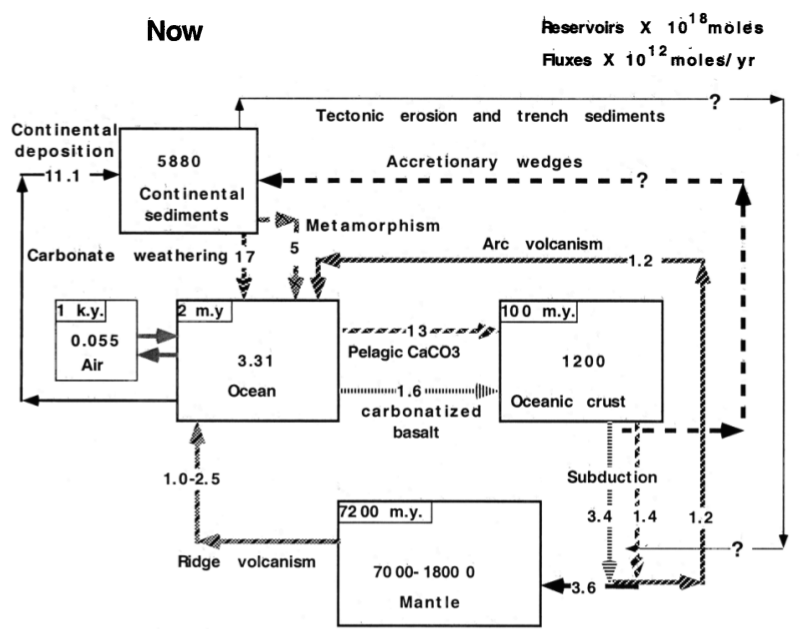
\includegraphics[scale=0.5]{Figures/ModelSNH.png}
  \label{FIG:ModelSNH}
  \caption{A comprehensive reservoir model of carbon cycle proposed by ~\citet{SNH-ZK:2001}. Current residence times are shown in the corners of each reservoir. Fluxes with poor constraints are also included.}
\end{figure}

\begin{figure}[h!]
  \centering
  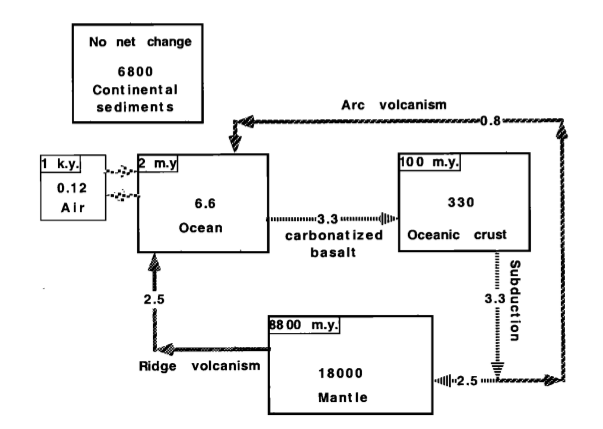
\includegraphics[scale=0.5]{Figures/SimplifiedModelSNH.png}
  \label{FIG:SNHZKBoxModelDiagramSimple}
  \caption{A simplified reservoir model of carbon cycle proposed by ~\citet{SNH-ZK:2001}. The atmosphere and oceans are treated as a single reservoir. Residence times are shown in the corners of each reservoir.}
\end{figure}

\begin{figure}[h!]
  \centering
  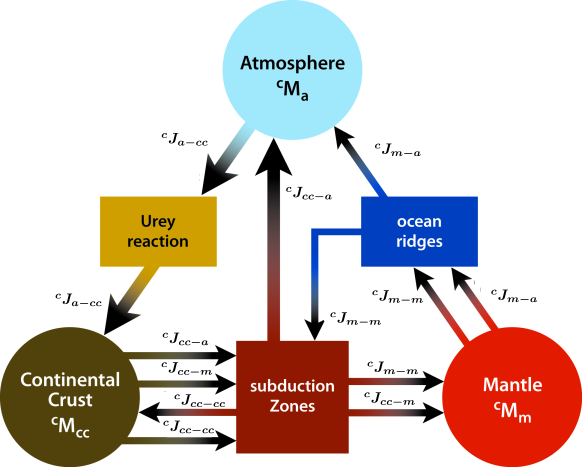
\includegraphics[scale=0.5]{Figures/RelabelJaniceFlowDiagram.png}
  \caption{A flow diagram showing the different reservoirs and pathways in our own constructed reservoir model of deep Carbon cycle.}
  \label{Fig:ReservoirFlowDiagram}
\end{figure}

%Although the atmosphere presently contains a small fraction of Earth's carbon inventory, ~\citet{KJD:2002} suggests the possibility of a significant fraction of Earth;s initial carbon inventory residing in the atmosphere. Scaling the carbon concentration of Venusian atmosphere to that of Earth's atmosphere based on their mass ratios, gives an estimated value of carbon in Earth's early atmosphere is $^cM_a(t_0) = 1.28 \time 10^8$ Gt. Alternatively, Earth's early atmosphere may have resembled today's atmosphere with an estimated value of carbon presently is $^cM_a(t_0) =\, ^cM_a(t_p) = 8.5 \times 10^2$ Gt ~\cite{NOAA:2017}. In both cases, Urey reaction plays an important role by transferring carbon from the atmosphere into the oceans where calcium carbonates precipitate ~\cite{UHC:1952}. 





% which was subsequently drawn down until cooling of global magma ocean and then further drawn down as the continental crust was being built. ~\citet{KJD:2002} estimates that this drawdown before reaching quasi-steady state could of been completed by the end of Archean or 1.5Ga ago at the latest. Alternatively, the atmosphere may have contained only a small fraction of the Earth;s carbon inventory thoughout its history with the Urey reaction as an important controlling process on the flux rate of carbon from the atmosphere to the continental crust. The source of the carbon in this model is associated with the mantle due to a higher flux of carbon release from volcanism in comparison to the flux of carbon subducted.


%\section{Reservoirs and Fluxes}
%Carbon has been partitioned into five main reservoirs: the core, the mantle, the continental crust, the oceans, and the atmosphere.

\subsection{Core}
	\begin{enumerate}
		\item Carbon is a siderophile element with a very large alloy/silicate partition coefficient~\cite{DR-CH-SN:2013}.
	\end{enumerate}
\subsection{Mantle}
	\begin{enumerate}
		\item Metamorphism, reverse Urey reaction
		\item Melting/Volcanism
		\item Subduction
		\item Removal of Carbon due to large alloy/silicate partition coefficient
	\end{enumerate}
\subsection{Continental Crust}
	\begin{enumerate}
		\item Weathering of exposed calcium bearing silicate rocks from acidic rain with dissolved carbon results in an outflux of calcium cations, silicates, carbonic acid and other chemicals transported by river systems into the oceans. This process is driven by the Urey reaction.
	\end{enumerate}
\subsection{Oceans}
	\begin{enumerate}
		\item Silicate weathering generates an influx of calcium and carbonic acid.
		\item Hydrothermal vents play a role in the percipitation of inorganic carbonates.
		\item Formanifera, diatoms life cycle results in deposition of calcite onto the ocean floor.
		\item Mid-Ocean ridge volcanism
		\item Subduction processes
		\item Serpentenization
	\end{enumerate}
\subsection{Atmosphere}
	\begin{enumerate}
		\item Carbon is comparatively insoluble with respect to other volatiles~\cite{HMM:2016}.
	\end{enumerate}

\section{Methods}

We first consider the mantle reservoir. We assume that carbon can be added to the mantle from the atmosphere early in Earth's history. This is the hypothesis set forth by Sleep and Zahnle (2001). Since little is known about the time dependence of this process we assume that the rate of mass addition decays exponentially with the age of the Earth. We also assume there is no significant transfer of carbon between the mantle and continental crustal reservoirs. This is consistent with association of carbon in the continental crustal reservoir and carbon in the atmosphere.

With these assumptions the mass of carbon in the mantle reservoir $M_{cm}(t)$ is given as a function of time by

\begin{equation}
  M_{cm}(t) = M_{cm0} + (M_{cmp} - M_{cm0}) (1 - e^{-\frac{t}{\tau_{am}}})
\end{equation}

where time is measured forward from the time of core formation ($t=0$) to the present ($t=4.4$ Gyr). The initial mass of carbon in the mantle is $M_{cm0}$, the present mass of carbon in the mantle is $M_{cmp}$, and the time constant for the loss of carbon from the atmosphere to the mantle is $\tau_{am}$. There is considerable uncertainty in the value of $\tau_{am}$ but on the basis of our previous discussion we take $\tau_{am} = 2 \times 10^8$ yrs.

We also require that the total mass of carbon in the three large reservoirs be constant over time. This balance between $t=0$ and $t_p$, requires that

\begin{equation}
  M_{cm0} = M_{cmp} + M_{cccp} - M_{ca0}
\end{equation}

where $M_{ca0}$ is the mass of carbon in the atmosphere at $t=0$ and $M_{cccp}$ is the mass of carbon in the continental crust at $t=t_p$. The continental crust did not exist at $t=0$ so that $M_{ccc0}=0$. As we have discussed the present mass of carbon in the atmosphere is negligible compared with the carbon masses in the mantle and the continental crust so that it is appropriate to take $M_{cap}=0$ in our mass balance. Eliminating $M_{cm0}$ we obtain an expression for the mass of carbon in the mantle as a function of time

\begin{equation}
  M_{cm}(t) = M_{cmp} + M_{cccp} - M_{ca0} + (M_{ca0} - M_{cccp}) (1 - e^{-\frac{t}{\tau_{am}}})
\end{equation}

To obtain the dependence of $M_{cm}$ on time we must specify $M_{cmp}$, $M_{cccp}$, $M_{ca0}$, and $\tau_{am}$.


We next consider the continental crust reservoir. Our approach is based on the hypothesis that carbon in the continental crust was primarily extracted from the atmosphere through the application of the Urey equation shortly after the first formation of continental crust. We specify that the continental crust began to form at $t=t_{cc0}$. Prior to this time there was no carbon in the continental crust so that

\begin{equation}
  M_{ccc} = 0 \quad \text{for} \quad 0 < t < t_{cc0}
\end{equation}

For our analysis of the evolution of major carbon reservoirs we assume that at $t=t_{cc0}$ the mass of carbon in the atmosphere was equal to the present mass of carbon in the continental crust $M_{cccp}$. We model the loss of carbon from the atmosphere with the growth equation

\begin{equation}
    \frac{d M_{ccc}(t)}{d t} = \frac{1}{\tau_{acc}} [M_{cccp} - M_{ccc}(t)]
\end{equation}

which is valid for the period $t_{cc0} < t < t_p$ and has the initial condition $M_{ccc} = 0$ at $t = t_{cccp}$. The applicable solution of the growth equation is

\begin{equation}
    M_{ccc}(t) = M_{cccp} (1 - e^{-\frac{(t-t_{cc0})}{\tau_{acc}}} )
\end{equation}

The mass of carbon in the continental crust grows exponentially with a time constant $\tau_{acc}$.

Finally we consider the atmosphere reservoir. As previously stated the sum of the carbon masses in the three large reservoirs is constant. We first consider the time period $0 < t < t_{cc0}$. During this period we have $M_{ccc}=0$ so that we can write

\begin{equation}
    M_{ca}(t) = M_{ca0} + M_{cm0} - M_{cm}(t)
\end{equation}

since we require that the total mass of carbon in the three large reservoirs be constant over time between $t=0$ and $t_p$,

\begin{equation}
  M_{ca0} + M_{cm0} = M_{cmp} + M_{cccp}
\end{equation}

substitution gives 

\begin{equation}
    M_{ca}(t) = M_{cmp} + M_{cccp} - M_{cm}(t)
\end{equation}

and substitution of $M_{cm}$(t) gives

\begin{equation}
    M_{ca}(t) = M_{ca0} - (M_{ca0} - M_{cccp})(1 - e^{\frac{-t}{\tau_{ca}}})
\end{equation}

for the period $0 < t < t_{cc0}$.

We next consider the time period $t_{cc0} < t < t_{p}$. During this period a mass balance gives

\begin{equation}
    M_{ca}(t) = M_{cmp} - M_{cm} (t) + M_{cccp} - M_{ccc} (t)
\end{equation}

since for the large reservoir carbon mass balance we can take $M_{cap} = 0$. Substitution of $M_{cm}(t)$ and substitution of $M_{ccc}(t)$ gives

\begin{equation}
    M_{ca}(t) = (M_{ca0} - M_{cccp})e^{-\frac{t}{\tau_{am}}} + M_{cccp} e^{-\frac{(t-t_{cc0})}{\tau_{acc}}}
\end{equation}

for the period $t_{cc0} < t < t_p$.




\section{Discussion}
%In reservoir models, the mantle is often considered as a homogeneous reservoir however OIB and MORB samples show distinct groups plotted in $\eta_{Nd}$ versus $^{87}Sr/^{86}Sr$ ~\cite{WWM:2015}. Due to the volumetric differences on OIB and MORB volcanism, I propose subdividing the mantle into two reservoirs.

\newpage
\section*{References}
 
\bibliography{Prospectus}

\end{document}
